
%(BEGIN_QUESTION)
% Copyright 2006, Tony R. Kuphaldt, released under the Creative Commons Attribution License (v 1.0)
% This means you may do almost anything with this work of mine, so long as you give me proper credit

Elektrisk ledningsevne i metaller skyldes frie elektroner. Frie elektroner er altså {\it ladningsbærere} i metalliske stoffer.

Ledningsevne i halvledere skyldes enten elektroner i ledningsbåndet eller hull i valensbåndet. Pentavalente dopstoff tilfører elektroner like under ledningsbåndet, slik at termisk energi kan løfte dem inn i ledningsbåndet og gjøre dem til ladningsbærere. Dette gir en {\it N-type} halvleder:

$$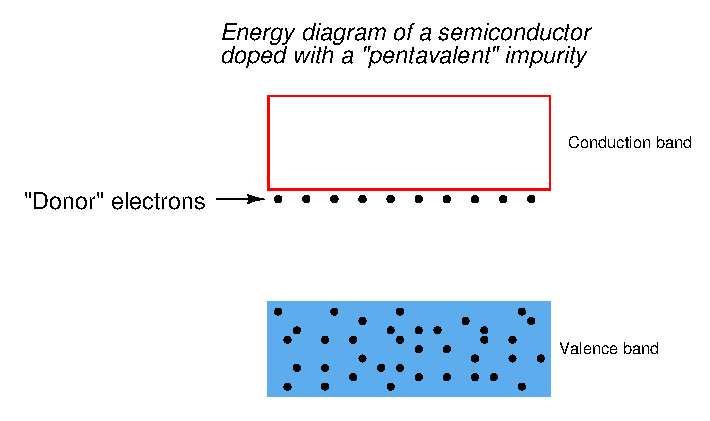
\includegraphics[width=15.5cm]{i00603x01.eps}$$

Trivalente dopstoff tilfører ``vakanser'' eller ``hull'' som valensbåndselektroner kan hoppe inn i ved hjelp av termisk energi. Dette muliggjør elektronbevegelse i valensbåndet, og vi kaller stoffet en {\it P-type} halvleder:

$$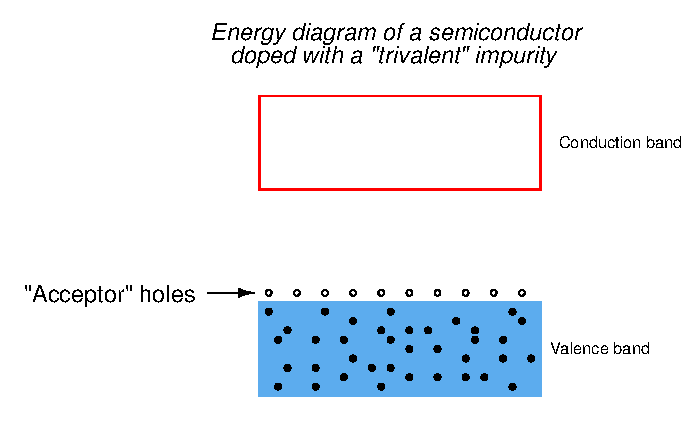
\includegraphics[width=15.5cm]{i00603x02.eps}$$

For å skille valensbånd-bevegelsen i P-type fra ledningsbånd-bevegelsen i N-type omtaler vi ofte valensbevegelsen i termer av ``hull'' og behandler disse som positive ladningsbærere.

\vskip 10pt

Ledning i væsker er annerledes. Siden molekylene kan bevege seg i væsker, kan hele molekyler være ladningsbærere dersom de er {\it ioniserte}. Forklar hva ``ionisering'' er, og skill mellom {\it anioner} og {\it kationer}.

\underbar{file i00603}
%(END_QUESTION)





%(BEGIN_ANSWER)

Et {\it ion} er et atom eller molekyl med elektrisk ubalanse; totalantall elektroner er ikke lik totalantall protoner.

%(END_ANSWER)





%(BEGIN_NOTES)

{\it Anioner} er ioner som tiltrekkes av positiv terminal (anode) i en elektrokjemisk celle. {\it Kationer} er ioner som tiltrekkes av negativ terminal (katode) i en elektrokjemisk celle.

%INDEX% Kjemi, ion: anion (definisjon)
%INDEX% Kjemi, ion: kation (definisjon)
%INDEX% Måling, analytisk: ledningsevne

%(END_NOTES)

